\chapter{宇宙学中的量子问题}
\label{chap:e23}

\begin{chapteropening}
前几章我们把望远镜对准一颗恒星、一个吸积盘、一次爆发——那些源你可以换个夜晚再看一遍，可以调带宽、可以重做实验。这一章的对象只有一个，而且只有一次：\textbf{整个宇宙}。它是一场早已发生、无法重启的光学实验，我们只是很晚才架起探测器，去读它留在天空上的一张底片。这张底片就是宇宙微波背景（cosmic microwave background，CMB）——一片几乎完美的黑体微波天空，上面叠着 \(10^{-5}\) 量级的温度花纹和更弱的偏振结构。

本章要回答三个层层递进的问题。第一，\textbf{这些花纹是从哪来的}？我们会看到它们的种子是暴胀期间被放大的\emph{量子}真空涨落，以及一个关键转折：这些量子涨落如何通过退相干（decoherence）"变成"可以用经典随机场描述的密度扰动。第二，\textbf{一束光跨越几十亿光年会经历什么}？它的偏振可能被悄悄转过一个小角，它的到达时间可能被介质和更深的物理拉开。第三，\textbf{我们能不能用一根宇宙学长的基线去称量最基本的物理}——洛伦兹不变性、光子的质量上限？把抽象的宇宙学，一步步落回本书熟悉的相干、偏振与光子到达时间上。
\end{chapteropening}

\section{宇宙作为一次不可重做的光学实验}
\label{sec:e23-lightfield}

先建立画面。谈 CMB 时人们张口就是"暴胀量子涨落"，但观测的入口其实非常朴素：望远镜先看到一个几乎完美的黑体微波天空，然后在这个平均背景上，去测一层薄薄的角向涨落。所以本节先把 CMB 当成一个\emph{光场}来称量，再一路退回到产生这些花纹的早期量子模式。

平均的 CMB 是一个温度 \(T_0=2.7255\pm0.0006\,{\rm K}\) 的黑体。第 \ref{chap:e05} 章把光场量子化、写出普朗克黑体公式，第 \ref{chap:e06} 章又专门讲了热态（thermal state）：一个热光场里每个频率模式的平均光子占据数由玻色分布给出，比强度再由普朗克公式给出：
\begin{equation}
  n_\nu=\frac{1}{\exp(h\nu/k_{\rm B}T_0)-1},
  \qquad
  I_\nu=\frac{2h\nu^3}{c^2}\,n_\nu .
  \label{eq:e23-planck-spectrum}
\end{equation}
\begin{formulaexplain}
\(n_\nu\) 是单个频率模式里的平均光子数，\(I_\nu\) 是黑体比强度。低频端 \(n_\nu\) 大，场接近经典热光；高频端 \(n_\nu<1\)，单模里常常连一个光子都不到。
\end{formulaexplain}
逐个符号落地：\(\nu\) 单位 Hz，\(h\) 是普朗克常数，\(k_{\rm B}\) 是玻尔兹曼常数，\(I_\nu\) 的单位是 \({\rm erg\,s^{-1}\,cm^{-2}\,Hz^{-1}\,sr^{-1}}\)（CMB 文献常换成 \({\rm MJy\,sr^{-1}}\)）。代两个真实频率进去感受一下：在 \(30\,{\rm GHz}\)，\(h\nu/k_{\rm B}T_0\simeq0.53\)，于是 \(n_\nu\simeq1/(e^{0.53}-1)\simeq1.4\)，低频通道仍是接近经典的热场；在 \(150\,{\rm GHz}\)，指数变大，\(n_\nu\simeq0.07\)，单模占据数已经小于 1。黑体强度峰落在 \(160\,{\rm GHz}\) 附近——这正是 Planck 高频仪器和许多地面实验把通道选在 \(90/150/220\,{\rm GHz}\) 的物理原因。FIRAS 把这个平均谱测得极其接近理想黑体，所以现代宇宙学干脆把平均谱当作\emph{已知背景}，把全部信息放进它上面的角向涨落和偏振里 \citep{1994ApJ...420..439M,1996ApJ...473..576F,2009ApJ...707..916F}。

把天空上的涨落展开成球谐（spherical harmonics），就像把一段声音展开成不同音高：
\begin{equation}
  T(\hat{\bm n})=T_0\,[1+\Theta(\hat{\bm n})],
  \qquad
  \Theta(\hat{\bm n})=\sum_{\ell m}a^{T}_{\ell m}\,Y_{\ell m}(\hat{\bm n}).
  \label{eq:e23-temperature-expansion}
\end{equation}
\begin{formulaexplain}
\(\Theta\) 是无量纲温度涨落，\(a^{T}_{\ell m}\) 是球谐系数，\(Y_{\ell m}\) 是球谐函数。这条式子把一张天空图拆成一层层角尺度：\(\ell\) 定尺度，\(m\) 管同一尺度上的方位花样。
\end{formulaexplain}
这里 \(\hat{\bm n}\) 是天空方向（一个单位矢量），多极矩 \(\ell\) 与角尺度近似满足 \(\theta\simeq180^\circ/\ell\)：\(\ell\simeq2\) 是半个天空那么大的花纹，\(\ell\simeq200\) 约一度，\(\ell\simeq2000\) 只有几角分。COBE 的差分微波辐射计首次在全天图上看到 \(\Delta T/T\sim10^{-5}\) 的结构，Planck 则把它一直分解到 \(\ell\sim2500\)。对一个各向同性的高斯天空，把同一个 \(\ell\) 上的 \(m\) 全部平方平均，就得到角功率谱（angular power spectrum）：
\begin{equation}
  \widehat C^{TT}_\ell=\frac{1}{2\ell+1}\sum_{m=-\ell}^{\ell}\bigl|a^{T}_{\ell m}\bigr|^2,
  \qquad
  D^{TT}_\ell=\frac{\ell(\ell+1)}{2\pi}\,C^{TT}_\ell .
  \label{eq:e23-cl-estimator}
\end{equation}
\begin{formulaexplain}
\(\widehat C^{TT}_\ell\) 是温度角功率谱估计量，来自一个 \(\ell\) 上全部 \(2\ell+1\) 个 \(m\) 模式的平均；\(D_\ell\) 是画图常用的重标度形式。这个平均就是 CMB 二点统计的核心压缩。
\end{formulaexplain}
若 \(a_{\ell m}\) 以 \(\mu{\rm K}\) 为单位，则 \(C_\ell\) 和 \(D_\ell\) 的单位是 \(\mu{\rm K}^2\)。\(D^{TT}_\ell\) 的第一声学峰在 \(\ell\simeq220\) 处，峰高约 \(5\times10^3\,\mu{\rm K}^2\)。这些峰不是随机的，它们来自复合（recombination）前光子—重子流体的\emph{声学振荡}：重子密度改变压缩峰的高度，暗物质密度改变引力势的衰减，角直径距离把物理声学尺度投影成天上的角尺度。Planck 用一个六参数的平直 \(\Lambda{\rm CDM}\) 模型拟合这些峰，给出 \(\Omega_bh^2\simeq0.0224\)、\(\Omega_ch^2\simeq0.120\)、\(n_s\simeq0.965\)、\(H_0\simeq67.4\,{\rm km\,s^{-1}\,Mpc^{-1}}\) 这样的典型精度 \citep{1992ApJ...396L...1S,1996ApJ...469..437S,2020A&A...641A...5P,2020A&A...641A...6P}。这里 \(\Omega_x\) 是第 \(x\) 种成分的无量纲密度参数（该成分密度与临界密度之比），\(h\equiv H_0/(100\,{\rm km\,s^{-1}\,Mpc^{-1}})\) 是约化哈勃常数，之所以写成 \(\Omega h^2\) 的组合，是因为 CMB 直接约束的是物理密度而与 \(H_0\) 的取值无关——这些都是六参数拟合的输出，若想细究记号的来历，可查任一本宇宙学教材，本书只把它们当作已知数字使用。

这里有一个"只有一次"的宇宙学专属限制。即使仪器完美无噪声，每个 \(\ell\) 上天空也只给你 \(2\ell+1\) 个 \(m\) 模式——样本就这么多，方差躲不掉。这叫宇宙方差（cosmic variance）：
\begin{equation}
  \frac{\sigma(C_\ell)}{C_\ell}=\sqrt{\frac{2}{(2\ell+1)\,f_{\rm sky}}} .
  \label{eq:e23-cosmic-variance}
\end{equation}
\begin{formulaexplain}
\(\sigma(C_\ell)/C_\ell\) 是样本方差带来的相对误差，\(f_{\rm sky}\) 是有效天区比例。低 \(\ell\) 可用模式少，所以大角尺度天生就有一层无法靠灵敏度消除的统计不确定性。
\end{formulaexplain}
\(f_{\rm sky}\) 是被使用的天空比例（银河面和强前景要被遮掉，故通常 \(f_{\rm sky}<1\)）。代数字：全天 \(\ell=2\) 的相对误差约 \(\sqrt{2/5}\simeq63\%\)，\(\ell=200\) 降到约 \(7\%\)，\(\ell=2000\) 只剩约 \(2.2\%\)。这就是为什么"低 \(\ell\) 反常""四极矩偏低"这类现象要放进有限模式数的协方差里判断，而不能只凭它在图上看起来显眼。这与第 \ref{chap:e15} 章的误差预算是同一种精神：先问"我到底有多少独立信息"。

偏振图比温度图多两个 Stokes 参数 \(Q\) 和 \(U\)。它们不是标量，而是随坐标旋转的\emph{自旋 2}（spin-2）量，所以要用自旋球谐函数展开，再线性组合成两种宇称明确的模式：
\begin{equation}
  (Q\pm iU)(\hat{\bm n})=\sum_{\ell m}a_{\pm2,\ell m}\,{}_{\pm2}Y_{\ell m}(\hat{\bm n}),
  \quad
  a^{E}_{\ell m}=-\tfrac12(a_{2,\ell m}+a_{-2,\ell m}),
  \quad
  a^{B}_{\ell m}=\tfrac{i}{2}(a_{2,\ell m}-a_{-2,\ell m}).
  \label{eq:e23-eb-definition}
\end{equation}
\begin{formulaexplain}
\(Q\pm iU\) 是自旋 \(\pm2\) 的偏振场，\({}_{\pm2}Y_{\ell m}\) 是自旋球谐函数，\(a^{E/B}_{\ell m}\) 是 E/B 模系数。这个组合把逐点的偏振方向翻译成全天上的两类图样。
\end{formulaexplain}
关键的物理在于宇称：\(E\) 模在镜像变换下像标量（偏振方向沿冷热斑呈放射或同心花样），\(B\) 模像赝标量（带旋涡感）。线性阶的标量密度涨落主要产生 \(T\) 和 \(E\)，\emph{不}直接产生原初 \(B\)。能产生 \(B\) 的只有几类：原初张量扰动（引力波）、弱引力透镜、偏振角被整体旋转、以及银河尘埃和同步辐射前景。记住这一点：\textbf{\(B\) 模是稀客}，谁能干净地造出它，谁就携带了最深的宇宙学信息。这条线索会在本章后面两次被拉动——一次指向原初引力波，一次指向偏振双折射。这两幅光场骨架图，见图~\ref{fig:e23-blackbody} 与图~\ref{fig:e23-power}。

\begin{figure}[tbp]
\centering
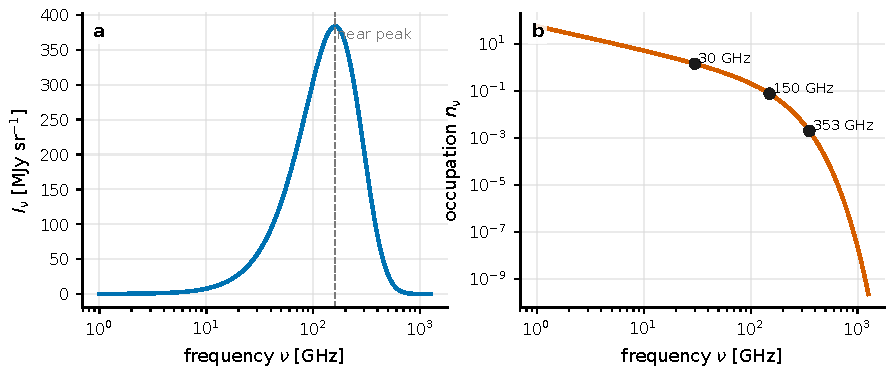
\includegraphics[width=0.9\linewidth]{figures/generated/chapter_16/ch16_cmb_blackbody.pdf}
\caption{CMB 的平均光场由黑体谱和模式占据数共同决定。左图把 \(T_0=2.7255\,{\rm K}\) 的普朗克谱写成 \({\rm MJy\,sr^{-1}}\)，峰值在 \(160\,{\rm GHz}\) 附近；右图是同一黑体在不同频率的单模平均光子数 \(n_\nu\)，低频通道占据数较高，高频通道逐渐进入 \(n_\nu<1\)。}
\label{fig:e23-blackbody}
\end{figure}

\begin{figure}[tbp]
\centering
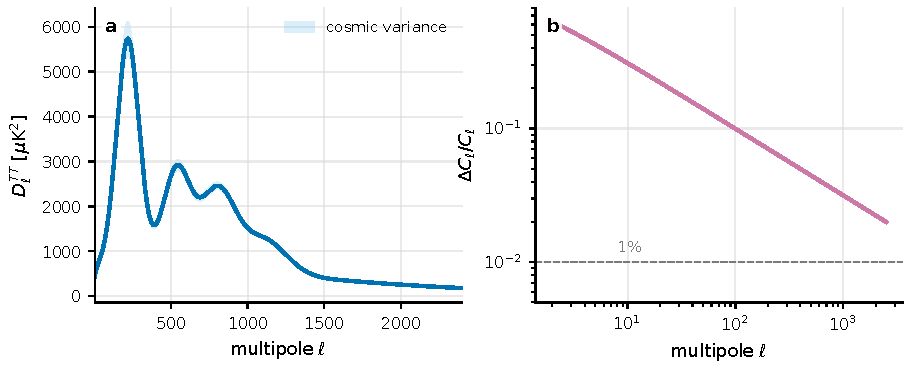
\includegraphics[width=0.9\linewidth]{figures/generated/chapter_16/ch16_cmb_power_spectrum.pdf}
\caption{角功率谱把天空涨落压缩到多极矩空间。左图是带声学峰和阻尼尾的 \(D_\ell^{TT}\)，阴影表示全天宇宙方差的量级；右图单独画出 \(\sqrt{2/(2\ell+1)}\)，说明大角尺度的误差由天上可用模式数决定，望远镜再灵敏也消不掉这部分方差。}
\label{fig:e23-power}
\end{figure}

\section{暴胀：把真空涨落放大成密度扰动}
\label{sec:e23-inflation}

上一节的 \(C_\ell\) 是天空上的统计量；暴胀（inflation）理论要解释的，是这些统计量为什么\emph{近似高斯}、\emph{近似尺度不变}、而且声学峰的相位是固定的（不是一团随机相位的杂波）。这里不能把 CMB 当成一束可反复制备的实验室光，而要把早期宇宙里每一个场模式，看成第 \ref{chap:e04} 章那个熟悉的量子谐振子——只不过它的频率随宇宙膨胀而变。

对标量曲率扰动 \(\mathcal R\)，人们定义一个把背景演化"打包"进去的 Mukhanov–Sasaki 变量 \(v\)：
\begin{equation}
  v(\bm x,\eta)=z(\eta)\,\mathcal R(\bm x,\eta),
  \qquad
  z=\frac{a\,\dot\phi}{H} .
  \label{eq:e23-ms-variable}
\end{equation}
\begin{formulaexplain}
\(v\) 是 Mukhanov–Sasaki 变量，\(\mathcal R\) 是我们最终关心的曲率扰动，\(z=a\dot\phi/H\) 把暴胀的背景演化装进一个系数里。用 \(v\) 写方程，每个傅里叶模就变成一个时变频率的量子谐振子。
\end{formulaexplain}
逐个符号：\(\eta\) 是共形时间（conformal time，满足 \({\rm d}\eta={\rm d}t/a\)），\(a\) 是尺度因子（无量纲，今天取 1），\(\phi\) 是驱动暴胀的背景标量场，\(H=\dot a/a\) 是哈勃率（单位 \({\rm s^{-1}}\)），点表示对宇宙时求导。把二阶作用量对每个傅里叶模 \(v_k\) 展开，就得到一条形式极其干净的运动方程：
\begin{equation}
  v_k''+\Bigl(k^2-\frac{z''}{z}\Bigr)v_k=0 .
  \label{eq:e23-ms-equation}
\end{equation}
\begin{formulaexplain}
\(v_k\) 是共动波数 \(k\) 的模式函数，撇号是对共形时间 \(\eta\) 的导数。方括号里 \(k^2-z''/z\) 就是这个"时变谐振子"的有效频率平方，符号的翻转正是暴胀的全部魔法所在。
\end{formulaexplain}
\(k\) 是共动波数（comoving wavenumber，单位 \({\rm Mpc^{-1}}\)）。这条方程的两种极限决定一切，逐一读出来：

\emph{亚视界}（\(k\gg aH\)）时，\(z''/z\) 相比 \(k^2\) 可忽略，方程退化成 \(v_k''+k^2v_k=0\)——一个普通简谐振子。取它的量子真空（Bunch–Davies 真空），归一化模式函数是
\[
  v_k(\eta)\simeq\frac{e^{-ik\eta}}{\sqrt{2k}} .
\]
这就是本书从头讲到尾的"最低能量态里仍在抖动"的真空涨落，只不过发生在早期宇宙的每一个短波模式上。

\emph{出视界}（\(k\simeq aH\)，之后 \(k\ll aH\)）时，膨胀把 \(z''/z\) 顶了上来并主导方程。此时增长解不再振荡而被\emph{冻结}，衰减解迅速缩小，于是 \(\mathcal R_k=v_k/z\) 趋于一个近似常数。"冻结"不是说模式停止演化，而是说相空间里一个方向被强烈压窄，最后只剩一个随机幅度，去支配后来的密度扰动 \citep{1988JETP...67.1297M,1990PhRvD..42.3413G,1996CQGra..13..377P}。

把这个冻结下来的二点统计，写成无量纲的原初曲率功率谱：
\begin{equation}
  \langle\mathcal R_{\bm k}\mathcal R_{\bm k'}\rangle
  =(2\pi)^3\delta^{(3)}(\bm k+\bm k')\,\frac{2\pi^2}{k^3}\,\mathcal P_{\mathcal R}(k),
  \qquad
  \mathcal P_{\mathcal R}(k)=A_s\Bigl(\frac{k}{k_*}\Bigr)^{n_s-1} .
  \label{eq:e23-primordial-spectrum}
\end{equation}
\begin{formulaexplain}
\(\mathcal P_{\mathcal R}\) 是无量纲原初曲率功率谱，\(A_s\) 是振幅，\(n_s\) 是谱指数（spectral index），\(k_*\) 是参考波数（pivot）。它把早期量子涨落的二点统计浓缩成今天 CMB 拟合里最核心的两个数。
\end{formulaexplain}
Planck 常取 pivot \(k_*=0.05\,{\rm Mpc^{-1}}\)，给出 \(\ln(10^{10}A_s)\simeq3.04\)，即 \(A_s\simeq2.1\times10^{-9}\)。谱指数 \(n_s=1\) 是精确的尺度不变；实测 \(n_s\simeq0.965\) 说明有一点"红倾"，长波略强于短波——这正是慢滚暴胀预期的微小偏离。请把这个数量级链条记牢：一个 \(10^{-9}\) 的原初曲率功率，经过辐射转移函数、声学振荡、复合面的有限厚度和后来的透镜平滑，被投影成今天天上 \(\Delta T/T\sim10^{-5}\) 的花纹 \citep{2020A&A...641A...6P,2020A&A...641A..10P}。

现在把它翻译成本书的量子光学语言。暴胀的时变背景，恰好把 \(\bm k\) 和 \(-\bm k\) 这一对模式，从真空演化成一个\emph{两模压缩态}（two-mode squeezed state）——第 \ref{chap:e06} 章介绍压缩态时说过，压缩就是"把一对模式的涨落成对放大，同时保持固定的相位关系"：
\begin{equation}
  |\psi\rangle=\prod_{\bm k}\exp\!\Bigl[\,r_k e^{-2i\varphi_k}\,\hat a_{\bm k}\hat a_{-\bm k}
  -r_k e^{2i\varphi_k}\,\hat a^\dagger_{\bm k}\hat a^\dagger_{-\bm k}\Bigr]\,|0\rangle .
  \label{eq:e23-squeezed-state}
\end{equation}
\begin{formulaexplain}
\(|\psi\rangle\) 是 \(\bm k\) 与 \(-\bm k\) 成对的两模压缩态，\(r_k\) 是压缩强度，\(\varphi_k\) 是压缩角，\(\hat a,\hat a^\dagger\) 是湮灭与产生算符。暴胀把真空涨落成对放大，并锁死它们的相位。
\end{formulaexplain}
每对模式的平均占据数是 \(N_k=\sinh^2 r_k\)。经过 \(50\text{--}60\) 个 e-folds（膨胀量级的对数）后 \(r_k\) 非常大，\(N_k\) 指数式增长。要提醒的是：这里的"占据数"指早期\emph{场模式}的量子激发数，和望远镜今天真正数到的 CMB 光子数不是一回事。在相空间里，压缩把 Wigner 函数拉成一条极细长的椭圆：一个方向被拉长（就是后来当作经典随机幅度的那个），另一个方向被压到很窄。正是这条被压死的方向，锁定了固定相位，从而在 \(TT\)、\(TE\)、\(EE\) 谱里排出一串规整的声学峰，而不是随机杂波（图~\ref{fig:e23-squeezed}）\citep{1990PhRvD..42.3413G,1996CQGra..13..377P,2006CQGra..23.2317P}。

\begin{figure}[tbp]
\centering
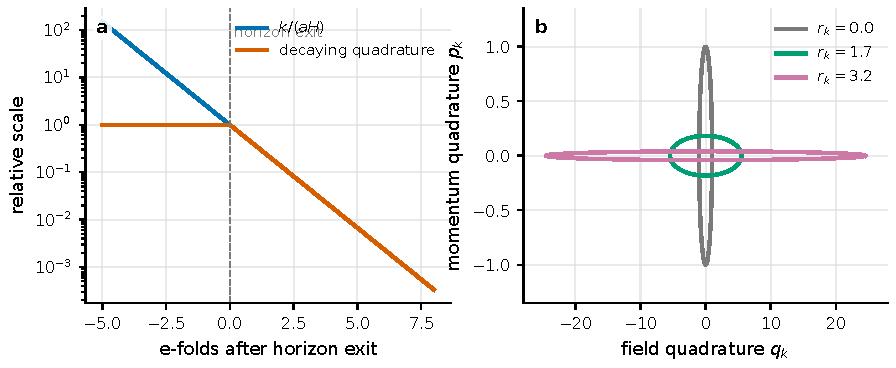
\includegraphics[width=0.9\linewidth]{figures/generated/chapter_16/ch16_squeezed_modes.pdf}
\caption{暴胀中的模式放大可以看成两模压缩。左图显示 \(k/(aH)\) 在穿出视界后指数下降，衰减方向被压窄；右图画相空间椭圆，\(r_k\) 增大时一个方向被拉长、另一个被压死，观测到的是后来表现为经典随机幅度的那条长轴。}
\label{fig:e23-squeezed}
\end{figure}

\section{退相干：量子涨落如何"变成"经典密度扰动}
\label{sec:e23-decoherence}

上一节留下一个不安：如果每个模式仍是一个纯的量子压缩态，它就是量子叠加，怎么能直接当成经典的密度涨落去算星系怎么长出来？答案是退相干（decoherence）。这也是本章第一个真正的"量子问题"：\textbf{一个被放大的量子态，为什么在观测上表现得像一个经典随机场}？

先给画面。一个量子态的"量子性"，藏在它密度矩阵的\emph{非对角项}里——那是不同幅度分支之间还能互相干涉的证据。可这些暴胀模式并不孤立：它们和一大堆没被观测的自由度纠缠在一起（未观测的短波模式、张量与标量的相互作用、复合前等离子体的自由度、透镜势，乃至数据分析里被边缘化掉的前景与仪器模式）。一旦把这些环境求和积掉，观测变量 \(q_k\) 的约化密度矩阵，非对角项就被一个高斯因子迅速压平：
\begin{equation}
  \rho_{\rm red}(q,q')=\rho_0(q,q')\,\exp\!\bigl[-\Gamma_k\,(q-q')^2\bigr] .
  \label{eq:e23-decoherence-density}
\end{equation}
\begin{formulaexplain}
\(\rho_{\rm red}\) 是观测变量 \(q_k\) 的约化密度矩阵，\(\rho_0\) 是未退相干的形式，\(\Gamma_k\) 衡量环境把非对角项压平的强度。当 \(q\ne q'\) 的相干项被压死，功率谱就可以用经典随机场去算。
\end{formulaexplain}
逐字读这条式子：\(q,q'\) 是同一个观测变量的两个不同取值，\((q-q')\) 越大代表两个分支相隔越远；指数因子 \(\exp[-\Gamma_k(q-q')^2]\) 是一口"钟形阀门"，把相隔较远的分支之间的干涉几乎完全关掉。\(\Gamma_k\) 的量纲取决于 \(q_k\) 怎样归一化，但物理判据很干脆：只要 \(\Gamma_k(\Delta q)^2\gg1\)，不同幅度分支之间就再也不会干涉，二点函数、角功率谱 \(C_\ell\)、角向三点谱（bispectrum）、透镜重建都可以按经典随机场老老实实地算。对暴胀模式，压缩越强、纠缠越深，\(\Gamma_k\) 越大，这个条件被极大幅度地满足——这正是"量子涨落变成经典密度扰动"这句话的精确含义。

要防止误解，说两句边界。退相干让\emph{统计}变经典，但它并没有替我们回答"到底是哪一个分支被实现了"——早期宇宙的"测量问题"在概念层面仍有争论。不过对我们能测的量（\(C_\ell\)、透镜重建、更高阶相关）来说，残留的相干相位信息太少，早已不足以撑起一次实验室式的 Bell 测试，也无法把 CMB 当成一个可反复制备的非经典态去操控 \citep{1996CQGra..13..377P,2006CQGra..23.2317P}。这与第 \ref{chap:e24} 章的量子网络望远镜恰成对照：那里你能主动制备、调制、重测量子态；这里，宇宙只给你一张不可重拍的底片，量子性早在复合之前就"沉淀"成了经典统计。

\section{涨落怎样产生：非高斯性与原初引力波}
\label{sec:e23-tensors}

二点函数（也就是 \(C_\ell\)）告诉我们\emph{有多少}涨落；要问这些涨落\emph{怎样产生}，得看两样更难测的东西：更高点函数（非高斯性）和张量模（原初引力波）。前者检验暴胀期间的相互作用与场内容，后者直指是否存在一份原初引力波背景。两者都极诱人，也都极易被有限模式数、透镜、尘埃和模板选择所限制。

若 \(\mathcal R\) 是严格高斯场，全部信息就都在二点函数里，三点及以上一律为零。可只要暴胀里有相互作用、非平凡声速、多场转移或尖锐特征，就会漏出非高斯性。它的主角是三点函数：
\begin{equation}
  \langle\mathcal R_{\bm k_1}\mathcal R_{\bm k_2}\mathcal R_{\bm k_3}\rangle
  =(2\pi)^3\delta^{(3)}(\bm k_1+\bm k_2+\bm k_3)\,B_{\mathcal R}(k_1,k_2,k_3) .
  \label{eq:e23-bispectrum}
\end{equation}
\begin{formulaexplain}
\(B_{\mathcal R}\) 是曲率扰动的三点谱（bispectrum），delta 函数强迫三个波矢首尾相接、闭合成一个三角形。三角形的\emph{形状}对应不同的早期宇宙相互作用，所以三点函数是非高斯性的主要语言。
\end{formulaexplain}
不同"形状"给出不同信号：local 型在\emph{扁长}三角形里最强（\(k_1\ll k_2\simeq k_3\)），equilateral 型在\emph{等边}三角形里最强，orthogonal 型是为区分不同相互作用而人为构造的近似正交模板。其中 local 型有一个很直观的实空间写法：
\begin{equation}
  \mathcal R(\bm x)=\mathcal R_g(\bm x)+\frac{3}{5}f^{\rm local}_{\rm NL}
  \Bigl[\mathcal R_g^2(\bm x)-\langle\mathcal R_g^2\rangle\Bigr] .
  \label{eq:e23-local-fnl}
\end{equation}
\begin{formulaexplain}
\(\mathcal R_g\) 是纯高斯场，\(f^{\rm local}_{\rm NL}\) 是 local 型非高斯的振幅。那个二次项让\emph{长波}去调制\emph{短波}的功率，所以 local 模板在扁长三角形里最敏感。
\end{formulaexplain}
\(f_{\rm NL}\) 无量纲。Planck 用温度加偏振给出 \(f^{\rm local}_{\rm NL}=-0.9\pm5.1\)、\(f^{\rm equil}_{\rm NL}=-26\pm47\)、\(f^{\rm orth}_{\rm NL}=-38\pm24\)（\(68\%\) 置信），都与零相容——没有发现标准模板下的显著非高斯性（图~\ref{fig:e23-nongaussian}）。这其实是对最简暴胀的一次有力支持：单场慢滚暴胀有一条"一致性关系"，预言扁长极限的 local 非高斯极小，数量级与 \(1-n_s\) 相当（也就是百分之几），\(f_{\rm NL}\) 天然就该很小 \citep{2003JHEP...05..013M,2020A&A...641A...9P,2020A&A...641A..10P}。

\begin{figure}[tbp]
\centering
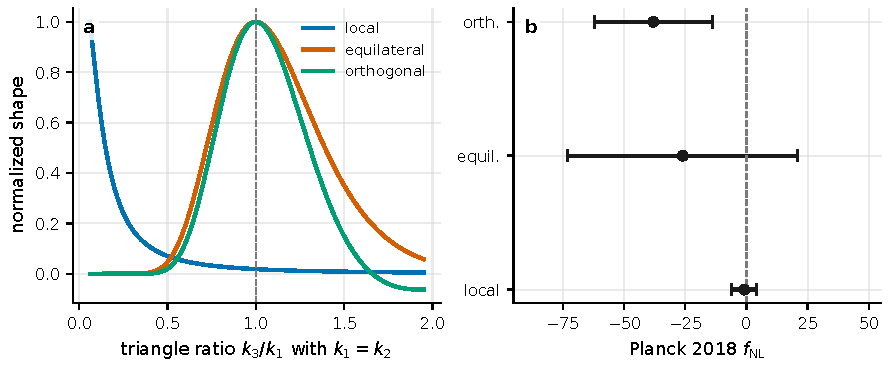
\includegraphics[width=0.9\linewidth]{figures/generated/chapter_16/ch16_non_gaussian_templates.pdf}
\caption{非高斯性由三角形构型和振幅共同决定。左图用 \(k_1=k_2\) 的切片比较 local、equilateral 与 orthogonal 三种模板的形状；local 型在扁长极限增强，equilateral 型在三边接近相等时最大。右图给出 Planck 对三个常用 \(f_{\rm NL}\) 的代表性约束，误差条都与零相容。}
\label{fig:e23-nongaussian}
\end{figure}

张量扰动是量子引力背景最直接的 CMB 目标——它就是暴胀产生的原初引力波，会在偏振里留下那位"稀客" \(B\) 模。人们用张量与标量功率之比来度量它：
\begin{equation}
  r(k_*)=\frac{\mathcal P_t(k_*)}{\mathcal P_{\mathcal R}(k_*)},
  \qquad
  \mathcal P_t(k)=A_t\Bigl(\frac{k}{k_*}\Bigr)^{n_t} .
  \label{eq:e23-tensor-r}
\end{equation}
\begin{formulaexplain}
\(r\) 是张量功率谱与标量曲率功率谱在 pivot \(k_*\) 处之比，\(\mathcal P_t\) 用振幅 \(A_t\) 和张量倾斜 \(n_t\) 描述。它把原初引力波背景压成 CMB 的 \(B\) 模搜索最常引用的一个数。
\end{formulaexplain}
\(r\) 无量纲，但 pivot 常取 \(0.002\) 或 \(0.05\,{\rm Mpc^{-1}}\)，两者\emph{不能混用}。单场慢滚给出另一条一致性关系 \(n_t\simeq-r/8\)。\(r\) 之所以珍贵，是因为它直接换算成暴胀发生时的能量标度：
\begin{equation}
  V_*^{1/4}\simeq1.06\times10^{16}\,{\rm GeV}\Bigl(\frac{r}{0.01}\Bigr)^{1/4} .
  \label{eq:e23-inflation-scale}
\end{equation}
\begin{formulaexplain}
\(V_*^{1/4}\) 是暴胀时的能量标度，\(r\) 是张量标量比。注意那个\emph{四次方根}：即便 \(r\) 的上限改进一大截，能标约束也只缓慢收紧。
\end{formulaexplain}
这条式子默认爱因斯坦引力、标准慢滚和单一能标。Planck 单独给出 \(r_{0.002}<0.10\)（\(95\%\) 置信）；与 BICEP/Keck 的 \(B\) 模偏振联合后收到 \(r_{0.002}<0.056\)，对应 \(V_*^{1/4}<1.6\times10^{16}\,{\rm GeV}\)——已逼近大统一能标。BICEP/Keck 把 2018 季数据与 Planck、WMAP 联合，进一步给出 \(r_{0.05}<0.036\)，并指出目前的限制同时被透镜 \(B\) 模和银河尘埃卡着脖子（图~\ref{fig:e23-bmode}）\citep{2020A&A...641A..10P,2021PhRvL.127o1301A,2019JCAP...02..056A}。换句话说，抓那位"稀客"的难处不在灵敏度，而在于先把冒充它的透镜和尘埃一个个请出去。

\begin{figure}[tbp]
\centering
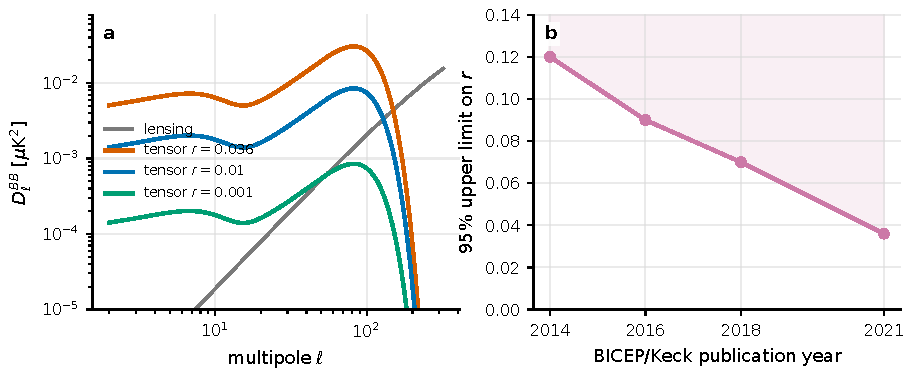
\includegraphics[width=0.9\linewidth]{figures/generated/chapter_16/ch16_bmode_constraints.pdf}
\caption{张量模式主要通过 \(B\) 模偏振受限。左图比较透镜 \(B\) 模与不同 \(r\) 的原初张量 \(B\) 模：\(\ell\sim80\) 的复合峰是地面实验的主战场，低 \(\ell\) 的再电离峰需要大天区。右图显示 BICEP/Keck 系列联合约束从 \(r<0.12\) 一路改进到 \(r_{0.05}<0.036\) 的量级。}
\label{fig:e23-bmode}
\end{figure}

\section{光子穿越宇宙：偏振会被悄悄转过一个角}
\label{sec:e23-birefringence}

前几节都在讲"底片是怎么曝光的"。现在换个视角：光从最后散射面出发，走了近乎整个宇宙的年龄才到我们这里，\textbf{一路上它自己会不会被改写}？第一个可被精密检验的效应，是偏振双折射（cosmic birefringence）——如果存在一种极轻的、像轴子（axion）那样的场耦合到电磁场，光的线偏振方向会在传播中被整体转过一个小角 \(\beta\)。第 \ref{chap:e22} 章从暗物质与轴子的角度写过这种偏振通道；这里我们看它落到 CMB 上会遇到什么麻烦。

麻烦首先是一个\emph{标定}问题。把整片天空的偏振方向转过 \(\beta\)，会让一部分 \(E\) 模泄漏成 \(B\) 模，在 \(EB\)、\(TB\) 这两个本该为零的交叉谱里冒出信号。小角度下这个泄漏近似是
\[
  \frac{C_\ell^{EB}}{C_\ell^{EE}-C_\ell^{BB}}\simeq \tfrac12\tan 4\beta\simeq 2\beta .
\]
代入数字感受量级：\(0.35^\circ=6.1\times10^{-3}\,{\rm rad}\)，于是 \(2\beta\simeq1.2\%\)。这个百分之一的信号，恰好卡在一个尴尬的位置——大到能在 Planck 级全天数据里留下统计迹象，又小到\emph{任何}绝对偏振角标定不准、尘埃自身的 \(EB\)、通带失配或 beam 泄漏都能伪装成它。要命的是，一个真的宇宙旋转角 \(\beta\)，和探测器偏振角整体错标了 \(\alpha\)，在 \(EB/TB\) 里几乎沿同一个方向作用，只用 CMB 你测到的其实是 \(\alpha+\beta\)。分开二者的钥匙，是频率：宇宙学旋转对所有频率一视同仁，而银河前景的偏振随频率变化，探测器错标又是逐频率的仪器量。

Minami 与 Komatsu 正是用这把"频率钥匙"，借银河前景在不同频率上的不同表现，同时估计逐频率的仪器错标 \(\alpha_\nu\) 和宇宙旋转 \(\beta\)，得到 \(\beta=0.35\pm0.14^\circ\)，并把地面角标定约 \(0.28^\circ\) 的系统误差从最终误差里剥离出去。后续用 WMAP+Planck PR4、在 \(23\text{--}353\,{\rm GHz}\) 上加入尘埃 \(EB\) 模型的分析，给出近全天 \(\beta=0.342^{+0.094}_{-0.091}{}^\circ\)，显著性约 \(3.6\sigma\)，但偏振尘埃自身的 \(EB\)、低频同步辐射 \(EB\) 和独立角标定仍是主要限制（图~\ref{fig:e23-biref}）\citep{2020PhRvL.125v1301M,2022PhRvD.106f3503E,2022PhRvL.128i1302D,2022NatRP...4..452K}。若把它解释成轴子样场，旋转角来自场值在传播两端的差：
\begin{equation}
  \beta=\frac12\,g_{\phi\gamma}\,\bigl[\phi(t_0)-\phi(t_{\rm LSS})\bigr] .
  \label{eq:e23-axion-birefringence}
\end{equation}
\begin{formulaexplain}
\(\beta\) 是 CMB 偏振的全局旋转角，\(g_{\phi\gamma}\) 是场与光子的耦合常数，方括号是今天 \(t_0\) 与最后散射面 \(t_{\rm LSS}\) 之间的场值差。若旋转真来自轴子样传播效应，它应\emph{近似不依赖频率}。
\end{formulaexplain}
\(g_{\phi\gamma}\) 的单位是 \({\rm GeV^{-1}}\)，\(\phi\) 是从最后散射面到今天的有效场值。这条式子默认旋转近似各向同性、频率无关、且源自\emph{传播}而非发射面本征的 \(EB\)。反过来，频率依赖就是最好的诊断：若 \(\beta(\nu)\propto\nu^{-2}\)，那更像穿过磁化等离子体的 Faraday 旋转（第 \ref{chap:e21} 章的传播效应）而非轴子；若 \(\beta\) 随天区、红移或时间变化，就得把一个全局角推广成方向依赖或时间依赖的相关函数。这里的教学要点值得记住：\textbf{在宇宙学里，一个"信号"和一个"标定误差"常常长得一模一样，把它们分开靠的往往不是更灵敏的探测器，而是更聪明地利用频率、天区这些额外维度。}

\begin{figure}[tbp]
\centering
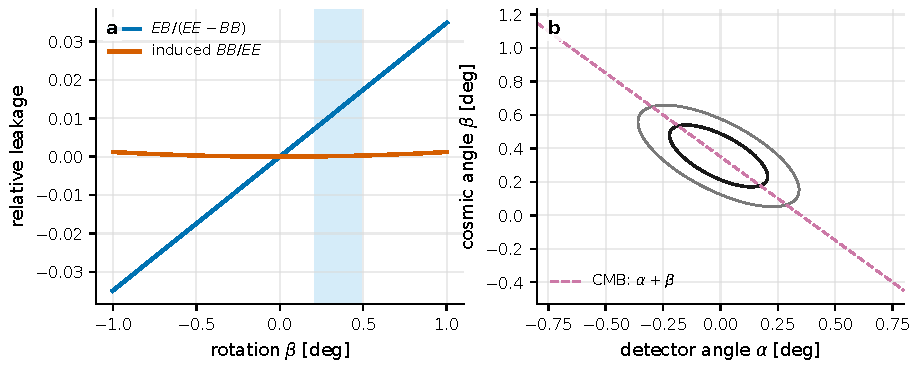
\includegraphics[width=0.9\linewidth]{figures/generated/chapter_16/ch16_birefringence_eb.pdf}
\caption{CMB 双折射把偏振角误差和宇宙学信号放进同一个平面。左图显示 \(\beta\) 对 \(EB\) 和诱导 \(BB\) 的小角度泄漏，阴影标出 \(\beta=0.35\pm0.14^\circ\) 的量级；右图显示探测器角 \(\alpha\) 与宇宙角 \(\beta\) 的退化方向：只用 CMB 时主要测到 \(\alpha+\beta\)，加入前景频率信息才可能把两者分开。}
\label{fig:e23-biref}
\end{figure}

\section{到达时间与色散：用宇宙学基线称量基本物理}
\label{sec:e23-timing}

偏振被转过一个角，是光在路上被改写的一种方式；\textbf{到达时间被拉开}，是另一种。这一节把本书最看重的两件工具——高时间分辨的光子事件表（第 \ref{chap:e13} 章）和瞬变源（第 \ref{chap:e20} 章的快速射电暴、伽马暴、脉冲星）——一起搬到宇宙学基线上，来检验最基本的物理：光速真的和频率无关吗？光子真的严格无质量吗？洛伦兹不变性在极高能量下还成立吗？

思路的核心，是一条比什么都朴素的判据：\textbf{如果一次爆发在同一瞬间发出了各种频率的光，而它们没有同时到达，那么"路上发生了事"}。要把这句话变成可测量，得写下频率与传播速度的关系。先看最熟悉、也最先要扣除的一项——星际与星系际的稀薄等离子体。一束电磁波在冷等离子体里满足的色散关系（dispersion relation）是
\begin{equation}
  \omega^2=\omega_p^2+c^2k^2,
  \qquad
  \omega_p^2=\frac{4\pi n_e e^2}{m_e}.
  \label{eq:e23-plasma-dispersion}
\end{equation}
\begin{formulaexplain}
\(\omega\) 是角频率，\(k\) 是波数，\(\omega_p\) 是等离子体频率，\(n_e\) 是电子数密度，\(e,m_e\) 是电子电荷与质量（CGS 制）。等离子体给色散关系加了一个\emph{常数项} \(\omega_p^2\)，波只有在 \(\omega>\omega_p\) 时才能传播。
\end{formulaexplain}
群速度（信号真正走的速度）是 \(v_g={\rm d}\omega/{\rm d}k\)。从 \eqref{eq:e23-plasma-dispersion} 解出 \(k=\sqrt{\omega^2-\omega_p^2}/c\)，两边对 \(\omega\) 微分再取倒数，一步不跳：
\[
  \frac{{\rm d}k}{{\rm d}\omega}=\frac{1}{c}\frac{\omega}{\sqrt{\omega^2-\omega_p^2}}
  \;\Longrightarrow\;
  v_g=\frac{{\rm d}\omega}{{\rm d}k}=c\,\frac{\sqrt{\omega^2-\omega_p^2}}{\omega}
  =c\sqrt{1-\frac{\omega_p^2}{\omega^2}}
  \simeq c\Bigl(1-\frac{\omega_p^2}{2\omega^2}\Bigr),
\]
最后一步用了 \(\omega_p\ll\omega\) 的泰勒展开 \(\sqrt{1-x}\simeq1-x/2\)。走过路径长度 \(L\) 的时间是 \(t=L/v_g\simeq(L/c)(1+\omega_p^2/2\omega^2)\)。于是两个频率 \(\omega_1<\omega_2\) 同时发出、到达时刻之差为
\begin{equation}
  \Delta t_{\rm plasma}
  =\frac{L}{2c}\,\omega_p^2\Bigl(\frac{1}{\omega_1^2}-\frac{1}{\omega_2^2}\Bigr)
  \;\propto\;\frac{\int n_e\,{\rm d}l}{\nu^2}
  =\frac{\rm DM}{\nu^2}.
  \label{eq:e23-dm-delay}
\end{equation}
\begin{formulaexplain}
\(\Delta t_{\rm plasma}\) 是等离子体色散造成的到达时差，与频率的\emph{平方成反比}，与沿视线积分的电子柱密度 \(\int n_e\,{\rm d}l\)（即色散量 DM，dispersion measure）成正比。低频光走得慢、到得晚。
\end{formulaexplain}
这正是第 \ref{chap:e20} 章里快速射电暴的招牌特征：一个毫秒脉冲在动态谱上被拉成一条 \(\nu^{-2}\) 的弯扫，测出这条弯扫的斜率就得到 DM，反过来还能称出一路上的电子。星际介质里 \(n_e\) 约 \(10^{-2}\text{--}10^{-1}\,{\rm cm^{-3}}\)，星系际更稀薄，但基线一长，柱密度可观，毫秒级的色散延迟稀松平常。

奇妙的是，\textbf{一个有质量的光子会给出结构一模一样的一项}。相对论色散关系是 \(E^2=(pc)^2+(m_\gamma c^2)^2\)——同样是给能量—动量关系加了一个常数项 \((m_\gamma c^2)^2\)，只不过这次是"静能"而不是"等离子体频率"：
\begin{equation}
  E^2=(pc)^2+(m_\gamma c^2)^2 .
  \label{eq:e23-massive-photon}
\end{equation}
\begin{formulaexplain}
\(E=h\nu\) 是光子能量，\(p\) 是动量，\(m_\gamma\) 是假想的光子质量，\(c\) 是（低频极限下的）光速。有质量光子的色散关系，和等离子体那一条在数学上完全同构——把 \(m_\gamma c^2\) 换成 \(\hbar\omega_p\) 就重合了。
\end{formulaexplain}
照搬上面的群速度推导（\(E\) 对应 \(\hbar\omega\)，\(p\) 对应 \(\hbar k\)）：\(v_g=\partial E/\partial p=pc^2/E=c\sqrt{1-(m_\gamma c^2/E)^2}\simeq c\,[1-\tfrac12(m_\gamma c^2/E)^2]\)，于是两个能量的到达时差是
\[
  \Delta t_{m_\gamma}=\frac{L}{2c}\,(m_\gamma c^2)^2\Bigl(\frac{1}{E_1^2}-\frac{1}{E_2^2}\Bigr)
  \;\propto\;\frac{1}{\nu^2}.
\]
它和等离子体延迟一样按 \(\nu^{-2}\) 走——这既是好消息也是坏消息。好消息：任何能测色散延迟的手段（射电脉冲星、快速射电暴）天生就能给 \(m_\gamma\) 定上限。坏消息：光子质量与等离子体的延迟\emph{完全退化}，必须靠独立测定的 DM（比如多条视线、多个源）把等离子体那份先扣干净，剩下的才可能归给 \(m_\gamma\)。判据依旧朴素：一次跨越宇宙学距离的爆发，若不同频率的主脉冲在扣除已知 DM 后仍\emph{一致到极高精度}，就把 \(m_\gamma\) 逼到极小的上限——基线 \(L\) 越长、时间分辨越细、频率跨度越大，这把尺子越狠。

第三种可能，藏在更高的能量里。若洛伦兹不变性在接近某个量子引力能标 \(E_{\rm QG}\) 时被极微弱地破坏（Lorentz invariance violation，LIV），色散关系会多出一个\emph{随能量增长}的修正项：
\begin{equation}
  E^2\simeq p^2c^2\Bigl[\,1\pm\Bigl(\frac{E}{E_{\rm QG}}\Bigr)^{n}\Bigr],
  \label{eq:e23-liv-dispersion}
\end{equation}
\begin{formulaexplain}
\(E_{\rm QG}\) 是洛伦兹破缺可能出现的能标（常拿普朗克能标当参照），\(n\) 是修正的幂次（\(n=1\) 线性、\(n=2\) 二次），\(\pm\) 表示高能光子可能走得更快或更慢。它与质量项的关键区别是：修正随能量\emph{升}高而变强。
\end{formulaexplain}
把 \eqref{eq:e23-liv-dispersion} 解出 \(p\simeq(E/c)[1\mp\tfrac12(E/E_{\rm QG})^n]\)，再取群速度 \(v=\partial E/\partial p\simeq c\,[1\pm\tfrac{n+1}{2}(E/E_{\rm QG})^n]\)，得到到达时差
\[
  \Delta t_{\rm LIV}\simeq\pm\,\frac{L}{c}\,\frac{n+1}{2}\,\frac{E_2^{\,n}-E_1^{\,n}}{E_{\rm QG}^{\,n}} .
\]
注意它的频率依赖和前两者\emph{正好相反}：等离子体和光子质量让\emph{低}频拖后腿（\(\propto\nu^{-2}\)），LIV 则让\emph{高}能光子领先或落后（\(\propto E^{n}\)）。这个符号与幂次上的差别，就是把三种效应拆开的抓手。所以检验 LIV 的天然对象是伽马暴和高能爆发：它们同时抛出低能与极高能光子，又在宇宙学距离外，\(L\) 与 \(\Delta E\) 都被拉到极致；只要在事件表里精确记下每个高能光子的到达时刻，再和低能光子对齐，就能把 \(E_{\rm QG}\) 顶到很高的下限。

把三条延迟并排看，本章的方法论就浮出来了（表~\ref{tab:e23-delays} 的口味）：同一套"高时间分辨事件表 + 宇宙学长基线"的观测，喂给三种不同频率依赖的模型，就能分别称量介质、光子质量与时空本身。这里我们不引用任何具体的数值上限——那属于实验前沿、且与选源和建模强相关；本节要教给你的是\emph{思路}：宇宙学距离不是障碍，它是把最微弱的基本物理效应\emph{放大}成可测到达时差的免费杠杆。第 \ref{chap:e13} 章那句"把每个光子的时间标签留在事件表里"，到这里终于显出它最大的野心——那根时间轴，长到可以量一量光子有没有质量、时空是不是严格洛伦兹不变。

\begin{table}[tbp]
\centering
\caption{三种到达时差的频率依赖各不相同，这正是把它们分开的抓手。}
\label{tab:e23-delays}
\begin{tabular}{@{}lll@{}}
\toprule
效应 & 色散关系里的多出项 & 到达时差随频率\\
\midrule
等离子体色散 & \(+\,\omega_p^2\)（\(\propto n_e\)） & \(\Delta t\propto \nu^{-2}\)，低频晚到\\
光子质量 & \(+\,(m_\gamma c^2)^2\) & \(\Delta t\propto \nu^{-2}\)，低频晚到（与等离子体退化）\\
洛伦兹破缺 & \(\pm\,p^2c^2(E/E_{\rm QG})^n\) & \(\Delta t\propto E^{n}\)，高能领先或落后\\
\bottomrule
\end{tabular}
\end{table}

顺带说一句相干性。到达时间被拉开的另一面，是相位记忆被打乱。第 \ref{chap:e02} 章讲过，一束光"还记得自己相位"的时间是相干时间 \(\tau_c\simeq1/\Delta\nu\)。当光穿过湍动的星际/星系际等离子体，多条略有不同的路径会让脉冲展宽、让相位在到达时被搅散，等效于把相干性磨损掉一部分——这正是第 \ref{chap:e21} 章传播效应要细算的散射。对本章而言，只需记住一个方向性的结论：\textbf{宇宙学距离既是放大微弱物理的杠杆，也是消磨相干与展宽脉冲的介质}；一台想在宇宙学基线上做精密计时或相干测量的仪器，必须同时把这两面写进它的误差预算（第 \ref{chap:e15} 章）。

\section{CMB 与光学量子天文学如何对接}
\label{sec:e23-bridge}

最后把这一章缝回全书。CMB 和前几部分的光学量子天文学，共享同一套"相关函数"的语言，但观测的含义天差地别——认清这个差别，才不会把两边的"量子"随手互换。

本书前半程反复用二阶相干函数 \(g^{(2)}\) 去刻画探测器时间序列里的强度涨落（第 \ref{chap:e08}、\ref{chap:e10} 章）：
\[
  g^{(2)}(\tau)=\frac{\langle I(t)\,I(t+\tau)\rangle}{\langle I\rangle^2}.
\]
它的时间延迟 \(\tau\) 和带宽 \(\Delta\nu\)，都是你可以\emph{主动挑}的。CMB 的基本二点函数则活在天球上，模式数由宇宙一次性发好：
\begin{equation}
  \langle X_{\ell m}\,Y^*_{\ell'm'}\rangle=C_\ell^{XY}\,\delta_{\ell\ell'}\,\delta_{mm'},
  \qquad
  X,Y\in\{T,E,B,\phi_{\rm lens}\}.
  \label{eq:e23-cmb-correlator}
\end{equation}
\begin{formulaexplain}
\(C_\ell^{XY}\) 是两个天空场 \(X,Y\) 的角功率谱，两个 Kronecker delta 表示在各向同性天空里不同 \(\ell,m\) 模式互不相关。这就是 CMB 版的二点相关函数。
\end{formulaexplain}
对照着读：\(g^{(2)}\) 的 \(\tau\) 与 \(\Delta\nu\) 由仪器主动设定，你可以换个延迟、换个带宽再测一遍；\(C_\ell\) 的模式数由宇宙给定，观测者只能改 sky mask、频率组合、beam、噪声权重和前景模型。CMB 没法像实验室那样调制源、重制备初态、重跑一次——它给的是早期场模式的统计信息，投影在 \(T/E/B\)、透镜与更高阶相关里的一份影子。

真正把这份影子变成宇宙学数字的，是地图级（map-level）的似然。所有频率图、偏振图和外部示踪都汇进同一个数据向量 \(\bm d\)：
\begin{equation}
  \bm d=\bm P\,[\,\bm s_{\rm CMB}(\bm\theta)+\bm s_{\rm fg}(\bm\eta)\,]+\bm n,
  \qquad
  -2\ln\mathcal L=(\bm d-\bm m)^{\mathsf T}\,C^{-1}\,(\bm d-\bm m)+\ln\det C .
  \label{eq:e23-cmb-likelihood}
\end{equation}
\begin{formulaexplain}
\(\bm d\) 是地图级数据向量，\(\bm P\) 是含 beam、mask、扫描策略与通带的观测/制图算子，\(\bm s_{\rm CMB}\)、\(\bm s_{\rm fg}\) 是宇宙信号与前景，\(\bm n\) 是噪声。似然把模型残差和总协方差 \(C\) 放在一起，就是从天空图推断宇宙学参数的工作形式。
\end{formulaexplain}
其中 \(\bm\theta\) 是宇宙学参数（如 \(A_s,n_s,\Omega_bh^2,\Omega_ch^2,r,\beta\)），\(\bm\eta\) 是前景参数（尘埃温度与谱指数、同步辐射谱指数、空间去相关等），协方差 \(C\) 一口气装下仪器噪声、样本方差、前景残差与校准不确定性。Planck、Simons Observatory 以及未来 CMB-S4、LiteBIRD 类实验的差别，主要就体现在 \(\bm P\)、\(C\)、频率覆盖、角分辨率和可控系统误差上 \citep{2016A&A...594A..13P,2016A&A...594A..20P,2017MNRAS.472.1195C,2019JCAP...02..056A,2020A&A...641A...6P}。

读 CMB 文献时，单位和 pivot 最坑人，临别叮嘱三句。其一，\(T_0\) 是 K，涨落图常用 \(\mu{\rm K}\)，而原初 \(\mathcal P_{\mathcal R}\) 无量纲——\(A_s\sim2.1\times10^{-9}\) 不能直接和 \(D_\ell^{TT}\sim5000\,\mu{\rm K}^2\) 比，中间隔着一整个辐射转移函数。其二，\(k\)（单位 \({\rm Mpc^{-1}}\)）和 \(\ell\)（角向模式数）通过 \(\ell\simeq k\,D_A(z_*)\) 相联，\(D_A(z_*)\) 是最后散射面的共动角直径距离。其三，\(r\) 的 pivot 不统一，\(r_{0.002}\) 和 \(r_{0.05}\) 不是同一个数，放开 \(n_t\) 时尤其不能混用。第 \ref{chap:e24} 章的量子网络望远镜会把讨论带回可以主动操控的实验系统；CMB 则站在相反的极限——初态不可重做，光路不可重置，可它把早期宇宙那场量子涨落留下的统计痕迹，工工整整地印在了一张我们今天才读到的底片上。

\section*{本章要点}
\addcontentsline{toc}{section}{本章要点}

\begin{itemize}
\item \textbf{CMB 首先是一个光场。} 平均是 \(T_0=2.7255\,{\rm K}\) 的黑体，信息在其上 \(\Delta T/T\sim10^{-5}\) 的角向涨落和偏振里；角功率谱 \(C_\ell\) 是核心二点统计，而低 \(\ell\) 有躲不掉的宇宙方差 \(\sqrt{2/[(2\ell+1)f_{\rm sky}]}\)。
\item \textbf{原初涨落的种子是量子的。} 暴胀把每个模式当成时变频率谐振子，出视界后曲率扰动被冻结；用量子光学语言，这是 \(\bm k\) 与 \(-\bm k\) 的两模压缩态，固定相位解释了成串的声学峰。
\item \textbf{退相干把量子变经典。} 与环境纠缠让约化密度矩阵的非对角项被 \(\exp[-\Gamma_k(q-q')^2]\) 压死，当 \(\Gamma_k(\Delta q)^2\gg1\)，功率谱就可按经典随机场计算——这就是"量子涨落变成经典密度扰动"的确切含义。
\item \textbf{高阶统计与张量模检验"怎样产生"。} \(f_{\rm NL}\) 与零相容，支持最简单场慢滚；\(r_{0.05}<0.036\) 把原初引力波（那位偏振里的 \(B\) 模稀客）压到能标 \(\lesssim1.6\times10^{16}\,{\rm GeV}\)，难点在于扣除透镜与尘埃。
\item \textbf{光在路上会被改写。} 偏振可能被转过 \(\beta\sim0.3^\circ\)（双折射），分离宇宙角与仪器角靠的是频率维度；到达时间可能被拉开，等离子体与光子质量给 \(\nu^{-2}\) 延迟且彼此退化，洛伦兹破缺给 \(E^{n}\) 延迟——频率依赖的不同，正是拆开它们的抓手。
\item \textbf{宇宙学距离是免费的杠杆。} 高时间分辨事件表（第 \ref{chap:e13} 章）配上宇宙学长基线与瞬变源，可把光子质量与洛伦兹破缺等最微弱的效应放大成可测的到达时差——代价是同一段距离也会消磨相干、展宽脉冲。
\end{itemize}

\medskip
\noindent\textbf{想一想。}
\begin{enumerate}
\item 全天 \(\ell=2\) 的宇宙方差相对误差约 \(63\%\)。若只观测半个天空（\(f_{\rm sky}=0.5\)），这个误差变成多少？为什么再灵敏的探测器也补不回这部分信息？
\item 等离子体色散和光子质量都给出 \(\nu^{-2}\) 的到达延迟。如果你手上有\emph{同一批}射电爆发在\emph{不同视线方向}的数据，你会怎样利用 DM 的变化，把可能的光子质量那一份从等离子体里剥出来？
\item 一个真实的宇宙偏振旋转 \(\beta\) 和探测器角错标 \(\alpha\)，在 CMB 里都表现为 \(EB\) 信号。为什么"用不同频率的前景"能把二者分开，而"把探测器做得更灵敏"不能？
\end{enumerate}
